\section{Progettazione}

\subsection{Layout}

Si è cercato di utilizzare un layout che si avvicina alla maggior parte dei 
siti web cosi che l'utente ha un senso di familiarità a prima vista.

Si può suddividere ogni pagina in quattro aree principali, 
partendo dall'alto verso il basso si può vedere

\begin{itemize}
	\item \textit{Header}:  visualizzerà i link alle pagine
	corrispondenti alle principali funzionalità del sito, compresi il login e la registrazione;
	\item \textit{Breadcrumb}: situato appena sotto l'header, tiene traccia del 
	percorso che fa l'utente visualizzandola e si può ritornare nelle posizioni precedenti;
	\item \textit{Main}: è il contenuto principale della pagina; in quanto
	tale occupa la maggior parte della larghezza del viewport a discapito
	della
	\item \textit{Footer}: la parte finale dove verrà visualizzata gli autori del sito web
\end{itemize}

\subsection{Accessibilità}

Per quanto riguarda l'accessibilità, si è prestato particolarmente attenzione a:

\begin{itemize}
	\item Testo alternativo per tutte le immagini presenti nel sito;
	\item Ogni parola di lingua straniera è segnalata con la sua appartenenza;
	\item I colori dei testi e sottofondo hanno un buon contrasto tra di loro;
	\item Il font utilizzato è chiaro e semplice;
	\item La struttura del sito è poco profonda, è possibile raggiungere ogni pagina
	del sito web con massimo tre click;
	\item I colori dei link visitati sono diversi da quelli non visitati;
	\item Il sito risponde ai ridimensionamenti, cambiando il design in base al dispositivo utilizzato
\end{itemize}

\begin{tabular}{| C{4.5cm} | C{4.5cm} | C{4.5cm} |}
		\hline
		\textbf{Testo} & \textbf{Sottofondo} & \textbf{Contrasto}\\
		\hline
		\#152238 & \#D0D0DC & 10.42\\
		\#551A8B & \#D0D0DC & 7.2\\
		\#152238 & \#FFFFFF & 15.93\\
		\hline
	\end{tabular}\\

\begin{figure}[H]
	\centering
	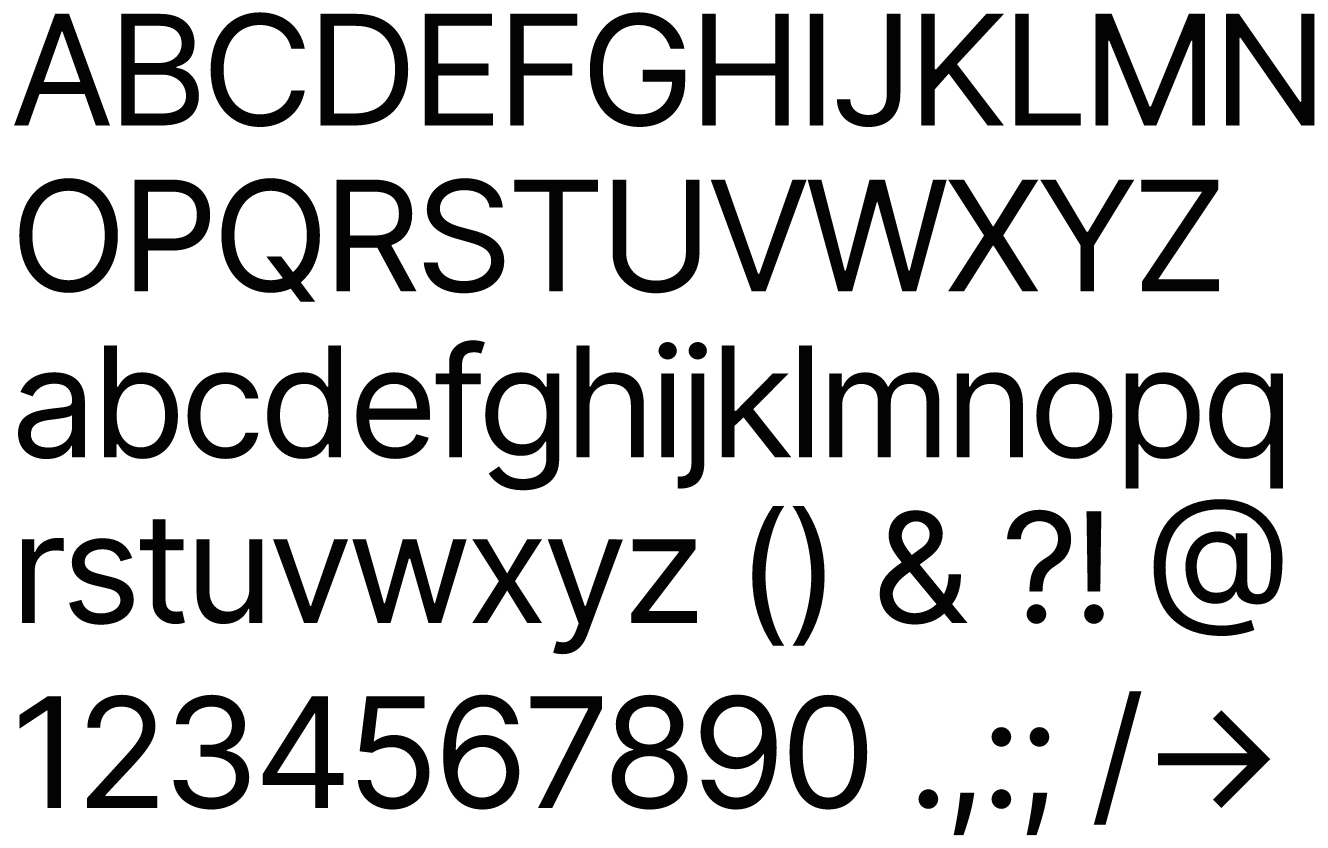
\includegraphics[scale=0.4]{res/font.png}
	\caption{Font Utilizzato}
\end{figure}